
% this file is called up by thesis.tex
% content in this file will be fed into the main document

%: ----------------------- introduction file header -----------------------
\chapter{Creation and Publication of Probabilistic Topic Models}\label{ch:scalability}

\graphicspath{{scalability/figures/}}

% -------------------------------------------------------------
% -- Scalability
% -------------------------------------------------------------

This chapter present \textit{\textbf{librAIry}}, our framework to create, publish and exploit probabilistic topic models through a service-oriented approach. In doing so, we reuse existing techniques and standards, which aim to make our results reusable and interoperable with other alternative approaches.


\section{Distributed Topic Modeling}


Numerous and varied are the domains where probabilistic topic models have been successfully used in recent years \citep{TapiNzali2017};\citep{ONeill2017};\citep{Greene2016};\citep{He2017}. Each one has its particularities. There are collections with only a few documents, and collections with thousands, and even millions, of texts. There are environments that only have a single machine to process the texts, and distributed environments with several dedicated servers. Taking into account such diversity, topic modeling algorithms have evolved to improve their efficiency in challenging situations, but they only cover the training phase of the model. The probabilistic topic model life-cycle begins with text pre-processing, continues with model training, follows with model distribution, and ends with model exploitation. In order to have a framework that covers the entire process of creating probabilistic topic models in both large- and small-scale, we have focused on adapting and reusing techniques and standards widely used in software engineering domain. 

\textit{librAIry} combines topic model training algorithms with natural language processing tools to  create models suitable for stand-alone use. The main objective is to facilitate the creation of reusable topic models by minimizing their technical and formatting dependencies. Methods and algorithms proposed in this thesis have been implemented and evaluated in this framework, which therefore serves as the technological basis for our research.

Our design requirements, which have guided our development process, can be organized into three categories:
\begin{itemize}
\item[Corpora representation requirements], which tackle the modeling of document collections and its metadata. This includes texts and their related annotations.
\item[Task distribution requirements], which refer to event management to notify changes in document collections. Coordination of this information is crucial for robust and reproducible results.  
\item[Process execution requirements], which capture the operations involved in creating a topic model. The parallel task execution leads to the creation of models.
\end{itemize}

The rest of the section describes how we have adapted existing techniques and standards in \textit{librAIry} to address each of the requirements categories described above. An open, distributed and scalable framework has been developed whose source code is publicly available for reuse\footnote{\url{https://github.com/librairy}}.

\subsection{Representing Corpora for Topic Modeling}

Inspired by a Staged Event-Driven Architecture (SEDA) based on message exchanges and status changes, our framework is articulated around three main concepts: \textit{resources}, \textit{actions} and \textit{states}. A \textit{resource} can be a \textit{document} that represents textual data (e.g. full-text of a research paper), or a logical \textit{part} of a textual data (e.g. the abstract section of a scientific article), or a \textit{domain} with a textual dataset (e.g. a conference proceedings) or even an \textit{annotation} made on them (e.g. review comments). An \textit{action} is an operation that can be performed on a resource (e.g. \textit{create}, \textit{update} or \textit{delete}). A \textit{state} is reached by a resource after an action is performed (e.g. \textit{created}, \textit{updated} or \textit{deleted}).  

To better illustrate this model, take the research articles published at the SIGGRAPH conference in 2016\footnote{\url{http://s2016.siggraph.org}}. First, a new \textit{document} is created for each article containing its full-text. Each document is then associated with several \textit{parts}, one for each section of the article. Finally, a \textit{domain} is created that groups all these \textit{documents} under the name of the conference. This initial representation can be extended by \textit{annotations} at different representation levels: at \textit{document level}, text based annotations such as named-entities, compounds or descriptive tags; at \textit{relational level}, comparison based annotations such as semantic similarity-based relations; and finally at \textit{domain level}, keyword based annotations such as tags or topics that describe the corpus.

\textit{Resources}, \textit{actions} and \textit{states} are individually addressable and linkable \cite{Turchi2012a} following the Linked Data principles\cite{Bizer2009}. Each of them has: (1) a name, (2) a retrievable (or dereferenceable) HTTP URI so that it can be looked up, (3) a descriptive information provided by using standard notation (e.g. JavaScript Object Notation (JSON)) when it is  looked up by URI, and (4) links to other URIs so that other resources can be discovered from it.


\begin{figure}
  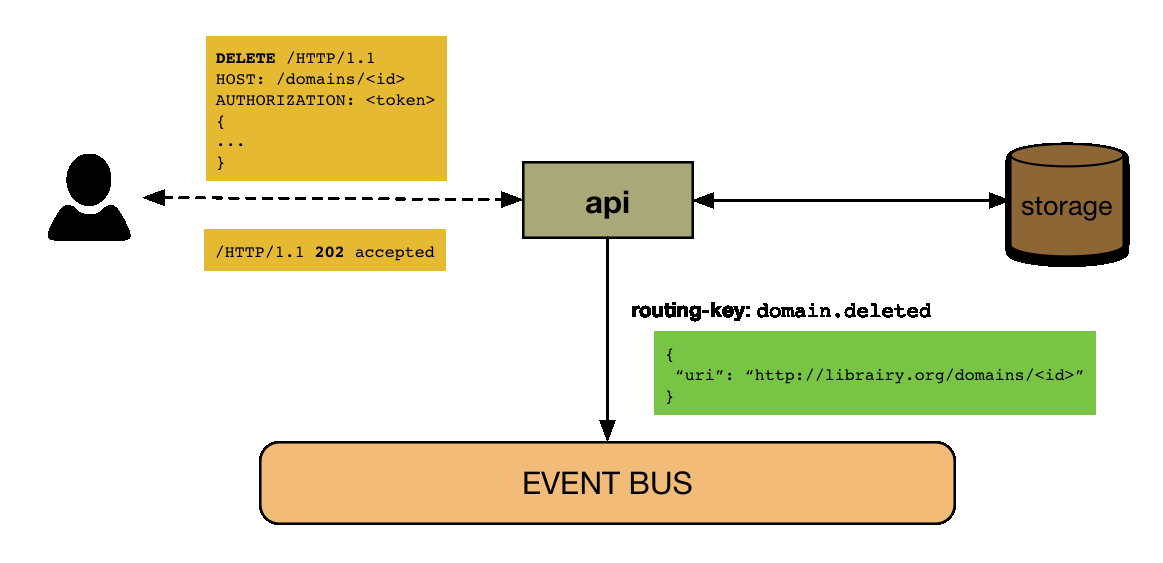
\includegraphics[scale=0.35]{api-domain-deleted}
  \caption{Domain deleted flow.}
  \label{fig:librairy-domain-deleted}
\end{figure}


\subsection{Event-oriented Processing Workflow}

Along with the resources mentioned above, there are two additional elements that provide a special behavior to the system: \textit{modules} and \textit{events}. An event is a message that notifies a new action performed on a resource. They are broadcasted so that any module is aware of the changes made to the resources. Modules are responsible for carrying out operations on the resources (e.g. tokenize a \textit{document} or create a topic model from a \textit{domain}). They can perform actions on one or more resources in response to a new state reached by a given resource. Actions that are paralleled by modules replicated through distributed environments.

The framework follows a publisher/subscriber approach where modules can publish and read \textit{events} to notify and to be notified about the state of a \textit{resource}. An event notifies a performed action (i.e. a resource and its new state), and follows the Representational State Transfer (REST)\cite{Fielding2002} paradigm. It contains the resource type and the new state reached by a specific resource ( i.e \textit{created}, \textit{deleted} or \textit{updated}). For example, when a new \textit{domain} is created, an \textit{event} message is published to the channel: $domain.created$. A channel is a space where events are published and modules can be subscribed to read the events. Events on a channel can be managed by one or more modules subscribed to that channel, that may perform an action (e.g. create a topic model when a domain have been created). Therefore, the workflow is not static and is not explicitly defined. A distributed workflow emerges according to the modules subscribed to the event channels.

We used the Advanced Message Queuing Protocol (AMQP) as the messaging standard to avoid any cross-platform problem and any dependency to the selected message broker (i.e the server that sends and receives messages). This protocol defines: \textit{exchanges}, \textit{queues}, \textit{routing-keys} and \textit{binding-keys} to communicate publishers (i.e message senders) and consumers (i.e message readers). Exchanges are like message inboxes, and queues subscribe to them by specifying the message types they are interested in (binding-key). A message sent by a publisher to an exchange is tagged with a routing-key. Consumers matching that routing-key with the binding-key used to link the queue to that exchange, will receive the message. This mechanism allows sending and receiving messages between consumers and producers by means of shared keys (i.e. routing-keys and binding-keys). A key follows the structure: \textit{resource.status}. Since a wildcard-based definition can be used to set the key, this paradigm allow modules both listening to individual type events (e.g. \'domains.created\' for new domains), or multiple type events (e.g. \#.created for all new resources).


\begin{figure}
  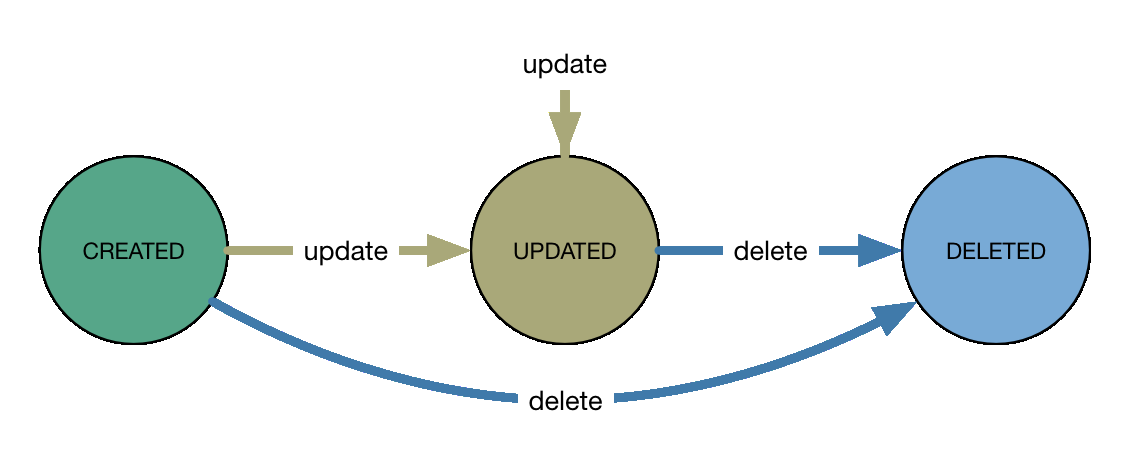
\includegraphics[scale=0.3]{resource-states}
  \caption{Resource states.}
  \label{fig:librairy-states}
\end{figure}


\subsection{Modular Execution Composition}

A module is a processing unit that reacts to events generated from resources. They have been designed following the microservices architectural style. A module is a cohesive, since it implements only functionalities strongly related to the concern that it is meant to model \cite{Dragoni2016}, and independent process working on the framework with a specific purpose. This purpose is defined by both the routing-key and the binding-key associated to the events handled by the module. 

There are three types of modules:
\begin{itemize}
	\item \textbf{Harvester}: creates resources such as \textit{documents} and \textit{domains}, from local or remote located textual files.
    \begin{itemize}[rightmargin=\dimexpr\linewidth-5cm-\leftmargin\relax]
    		\item Listening for: nothing
		\item Publishing to: \textit{document.(created)}, \textit{domain.(created;updated)}
    \end{itemize}
    \item \textbf{Annotator}: retrieves named-entities, compounds, lemmas and makes annotations resulting of Natural Language Processing (NLP) task execution from \textit{documents} and \textit{parts}.
    \begin{itemize}[rightmargin=\dimexpr\linewidth-5cm-\leftmargin\relax]
    	\item Listening for: \textit{document.(created;updated)}, \textit{part.(created;updated)}
		\item Publishing to: \textit{annotation.(created;deleted)}
    \end{itemize}
    \item \textbf{Modeler}: builds representational models from a given \textit{domain}. 
    \begin{itemize}[rightmargin=\dimexpr\linewidth-5cm-\leftmargin\relax]
    	\item Listening for: \textit{domain.(created;updated)}
		\item Publishing to: \textit{annotation.(created;deleted)}
    \end{itemize}
\end{itemize}

\begin{figure}
  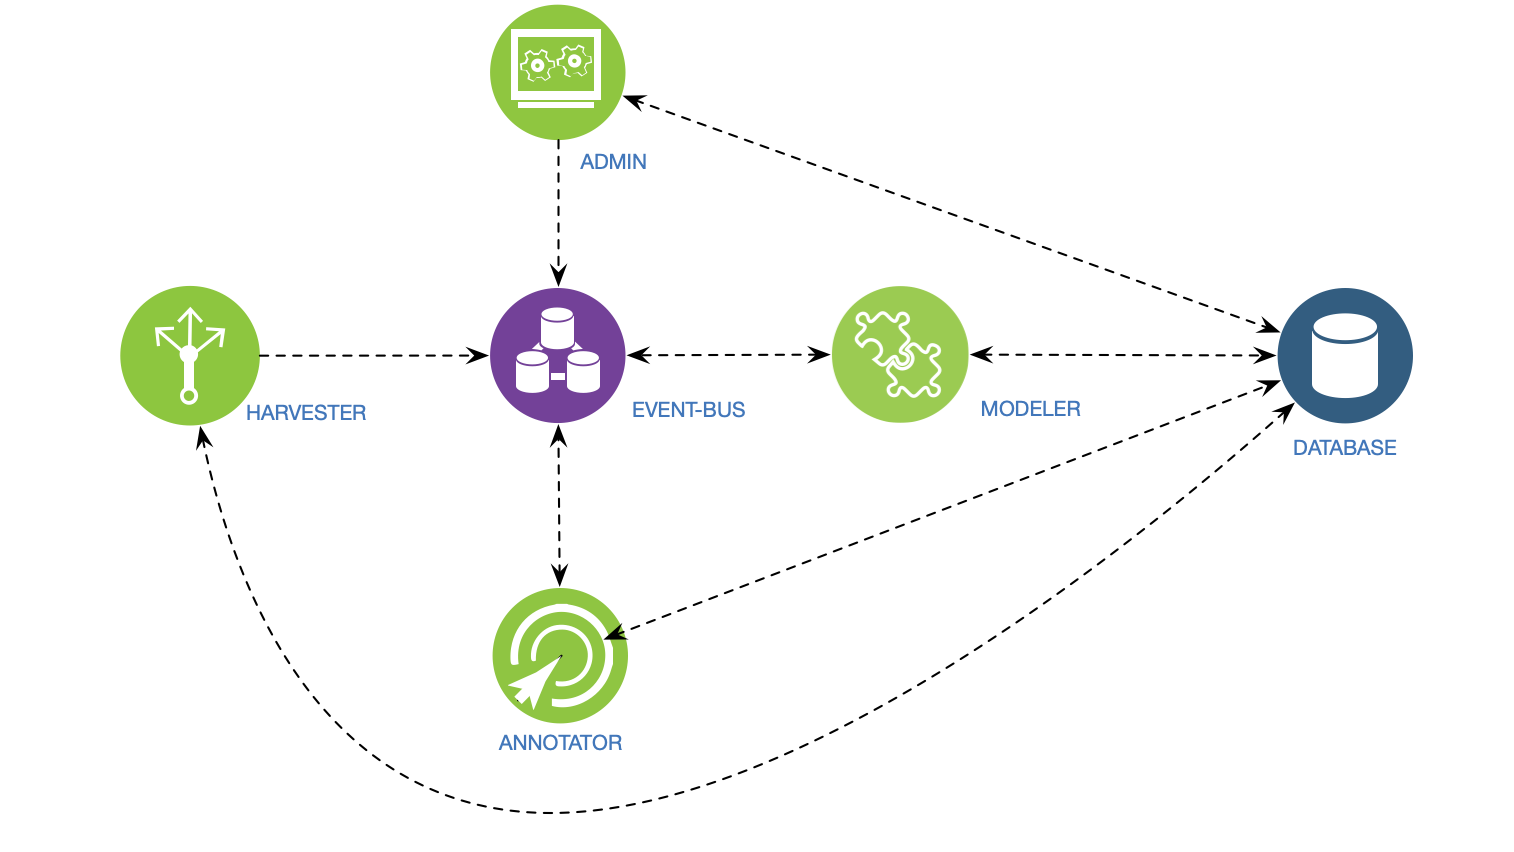
\includegraphics[scale=0.25]{modules}
  \caption{Modules.}
  \label{fig:librairy-modules}
\end{figure}


In addition to these modules, there is an end-user-oriented module, which offers a RESTful Application Program Interface (API) over HTTP. Any external operation motivated by a user is handled here. Some of them, usually those related to reading operations, are completely managed by this module getting all the data from the internal storage. However, those operations implying a modification of the status of some resource (e.g. creation of a \textit{document}), may be also performed by other modules listening for that type of event asynchronously. This module publishes to the following routing-keys: \textit{domain.(created;updated;deleted)}, \textit{document.(created;updated;deleted)}, \textit{part.(created;updated;deleted)}, and \textit{annotation.(created;updated;deleted)}.

Each module is wrapped with an Application Program Interface (API) over HTTP and TCP, for efficiency reasons. It follows the web standards for the RESTful API development over HTTP, and offers an Avro\footnote{\url{https://avro.apache.org}} protocol for TCP requests.  



\section{Probabilistic Topics Publication and Exploitation}



% existentes herramientas de análisis de textos: escalabilidad vertical

% en que consiste los modelos probabilísticos de tópicos para necesitar tareas de NLP


%In natural language processing, the term topic means a set of words. These are the words that come to mind when thinking of this topic. For example music could associate the words sound, instrument and composition. Without going more deep now, a topic model automatically discovers the words that are most likely to describe the topics present in a document collection. A trained model may then be used to infer which of these topics occur in new documents and can also pick out which portions of a document cover which topics.

%The learning process in a topic model first requires creating bag-of-words (BoW) from texts. A BoW contains the frequencies of each word in a text. The model uses these representations to discover the word distributions that best define the topics to fit their presences in the documents, assuming that a document can covers several topics. Take the following text: "Apple has just released in its Apple Store a video celebrating International Women's Day, about the lives of several relevant women, especially the most influential young woman in recent years.". A basic approach would transform that text into a BoW that considers whitespaces and punctuation marks as word separators (e.g. 'Apple'(2), 'has'(1), 'just'(1), etc). But this approach makes several mistakes. 'Apple' does not appear twice, but only once, as 'Apple Store' is different to 'Apple'. Some natural language processing tasks are needed to make these assessments. Using Named Entity Recognition (NER) techniques, for example,  'Apple', 'Apple Store' and 'International Women's Day' are different words in a BoW. Sometimes a normalization is applied to group plural and singular nouns. Using stemming techniques and Part-of-Speech (PoS) tagging, 'women' and 'woman' are transformed into a same word, 'woman', with a frequency equals to the sum of their frequencies, in this case 2. This is just a very simple illustration of how texts need to be processed to train probabilistic topic models. 

%While most topic model tools already include such functionality, they have not taken into account integration and scalability issues in their development. It is difficult, and sometimes impossible, to incorporate external resources into the workflow to perform some of these tasks (e.g. NER, PoS Tagging, etc) due to incompatibility problems. They can appear at the data level with different annotation categories (e.g. AnCora and CoNLL-U tagsets for PoS tagging), or at the execution level with different technological stacks (e.g. Java and Python). Furthermore, they are mainly focused on vertical scalability (better processing machines), instead of horizontal scalability (more processing machines). There are tools that have recently addressed, although only partially, some of these incompatibilities\footnote{\url{https://www.openml.org}}. But, as far as we know, these approaches keep forgetting the horizontal scalability in their designs. Only with high-performance machines can huge document collections be processed, instead of combining some lower-performance machines.

%We propose a distributed framework where multiple and heterogeneous text mining tools can collaboratively work. A shared workflow emerges to combine external tools (e.g. java-based and python-based tools to create topic models and NLP tasks), that may be located on different machines and even replicated at different scales. This raises both technical and functional challenges to coordinate distributed executions. From the technical point of view, isolated environments and communication mechanisms are required so dissimilar tools can be executed with maximum guarantees. From the functional point of view, all executions must be coordinated to reach a final result as aggregation of partial results derived from each execution.

 


%\subsubsection{Storage}

%Multiple types of data can be handled in this ecosystem. Inspired in the Data Access Object (DAO) pattern, we have created a Unified Data Manager (UDM) providing access to any type of data used in the system.  Three types of databases have been considered:
%\begin{itemize}
	%\item \textbf{column-oriented database}: Focused on unique identified and/or \textit{structured data}. This storage allow %us searching key elements across resources. 
	%\item \textbf{document-oriented database}: Focused on indexing raw text. This storage allow us to execute advanced search %operations over all the information gathered about a textual resource. 
    %\item \textbf{graph database}: Focused on relations. This storage allow us exploring resources through the relationships %between them.
%\end{itemize}


\section{Summary}

A distributed framework is proposed where existing algorithms and tools coming from different technologies can work collaboratively to process and analyze huge collections of textual resources. This approach has been successfully applied to some real world scenarios \footnote{\url{http://drinventor.dia.fi.upm.es}}.
 
A new model definition based on the previously mentioned principle of maximizing information re-usability and minimize irrelevant data has been studied to create a fine-grained resource design. New domains, in the sense of particular vocabularies or specific textual formats, have been also analyzed to be included into the system via specific harvesters or more precise annotators. Moreover, a template-based mechanism oriented to facilitate the integration of new tools and techniques into the system has been built to make easier to develop new modules as well as increasing the available modules in public repositories.

Our approach to create and inference probabilistic topics is \textbf{scalable} enough to work properly in both situations. This chapter presents a framework for processing topic models in document collections ranging from only a few texts, to large scale corpora. Methods and algorithms proposed in this thesis have been implemented and evaluated in this environment, which therefore serves as the technological basis for our research. The motivation is twofold, on the one hand to create a scalable system to analyze documents and discover topics, and on the other hand to create reusable topic models that can be easily integrated into that system.
